\documentclass[master.tex]{subfiles}
 
\begin{document}

\chapter{Float vs Double precision} \label{sec:float-vs-double}
\renewcommand{\thechapter}{A}
This appendix should serve as a small evaluation whether using float (4 byte; $\approx 7$ decimals) or double (8 byte; $\approx 16$ decimals) precision in the simulation has a notable impact on the results. A significant speedup may be achieved when using float operations thus if the numeric problem is not effected \textit{too much} by the lower precision it is preferable.\newline
For this assertion the first parameter set from \autoref{sec:polarization_equation_evaluation} is run in float precision and the results are compared, but only for 100,000 iterations. Then three different plots are made where the mean turbulent flow in the Core and \ac{SOL} region are compared. The plots differ by the iteration rage over which the mean value is taken. The plots show how much the \textit{float} evaluation differs from the \textit{double} evaluation. Every 20 iterations the the turbulent flow is calculated and saved. The differences are evaluated using $\frac{\Gamma_{double} - \Gamma_{float}}{\Gamma_{double}}$ and the the mean value is taken starting from three different time points. The error bars represent the standard deviation from the mean value of the considered deviations. 

\begin{figure}[!hbtp]
    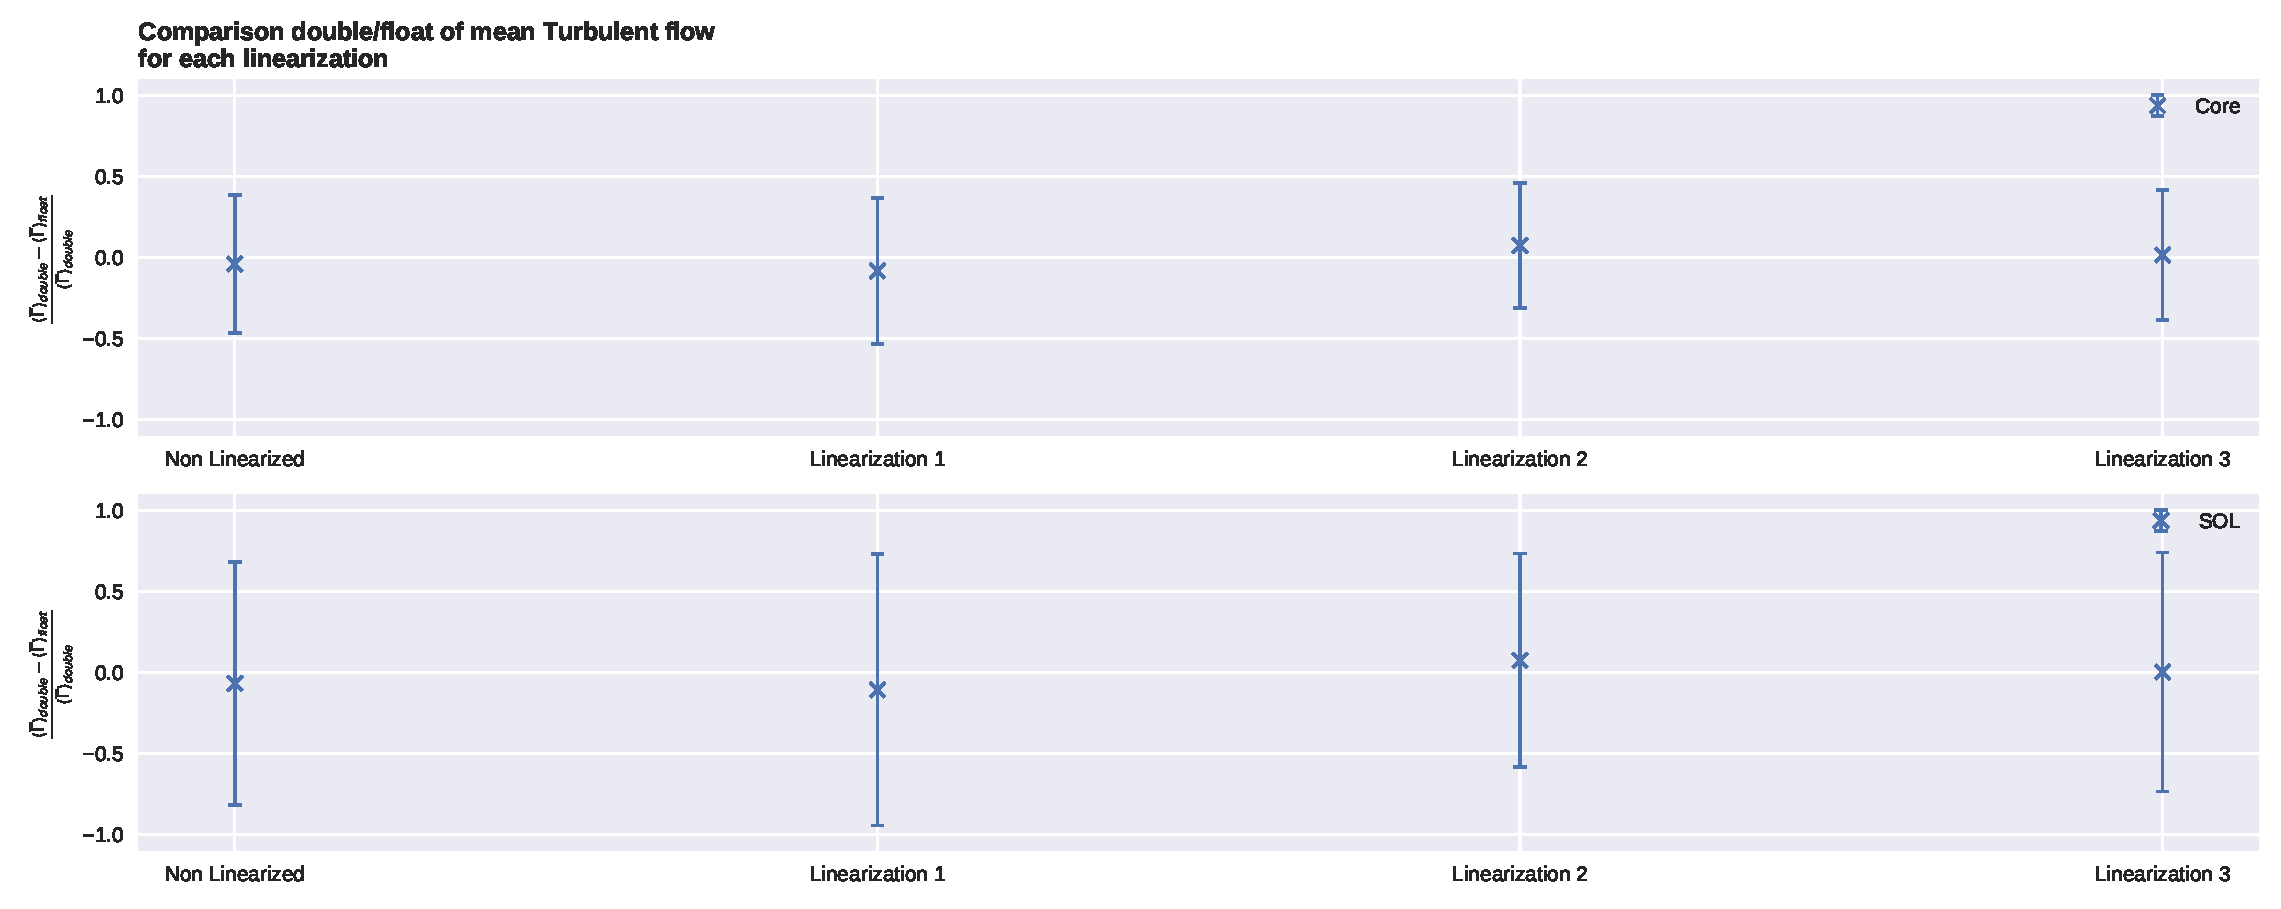
\includegraphics[width=0.32\linewidth]{pdfs/double_vs_float_all.pdf}
    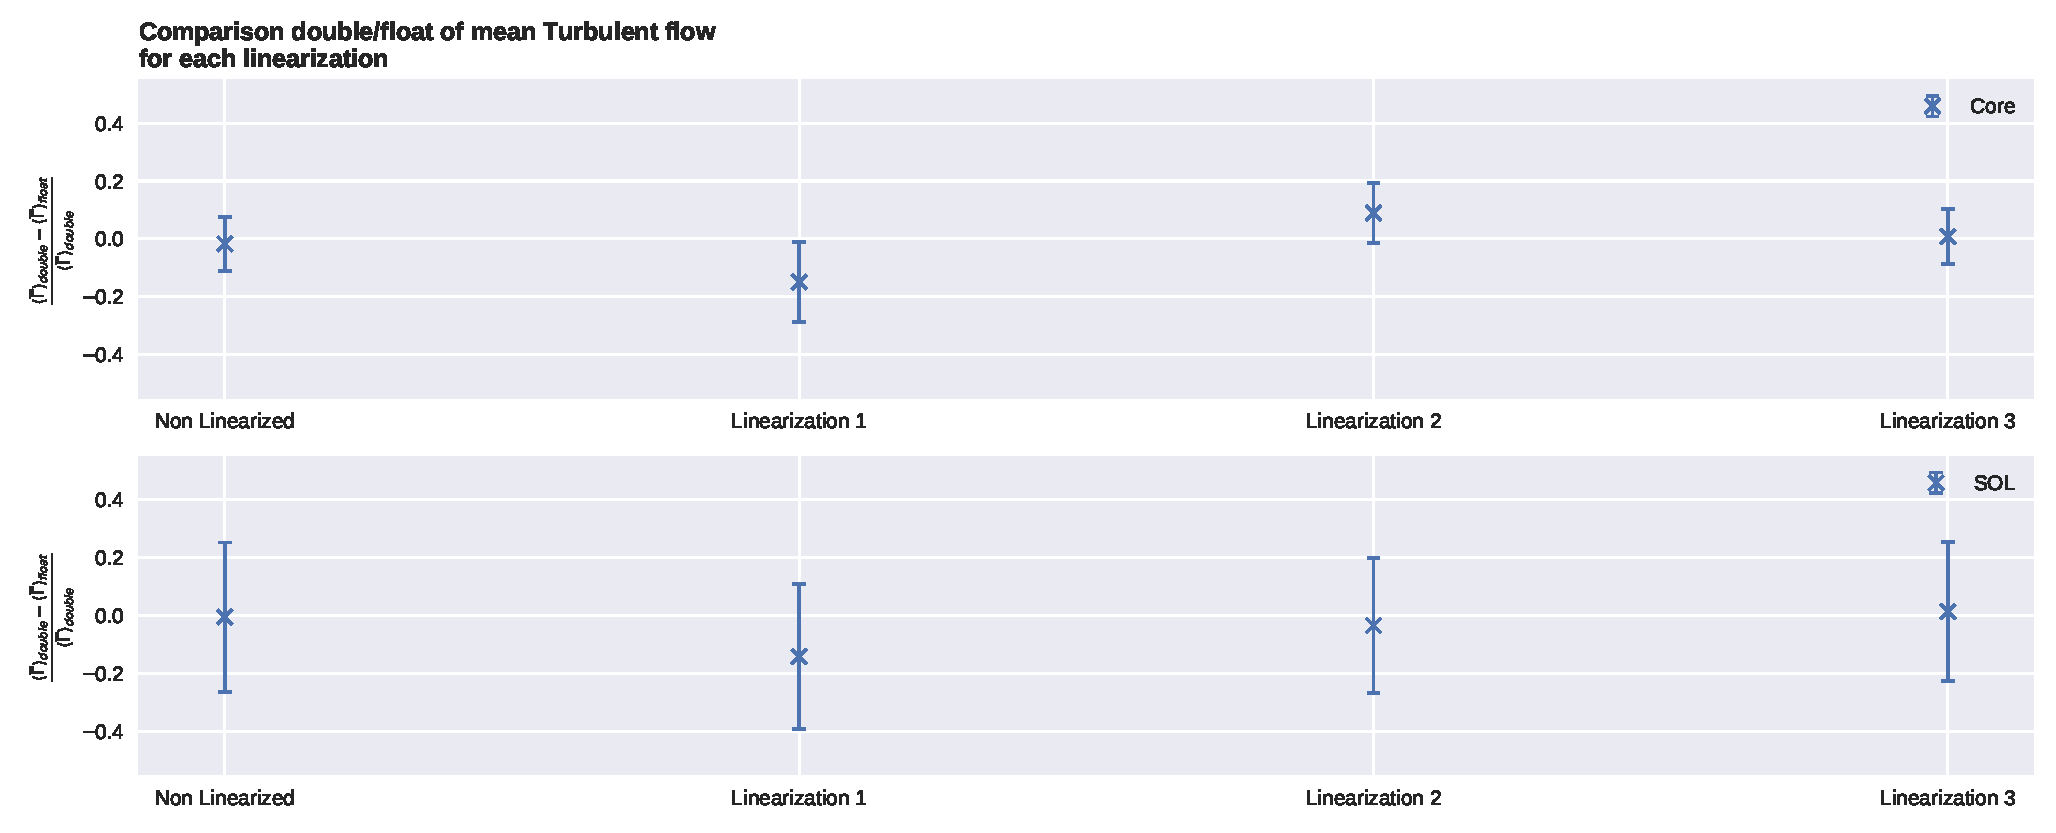
\includegraphics[width=0.32\linewidth]{pdfs/double_vs_float.pdf}
    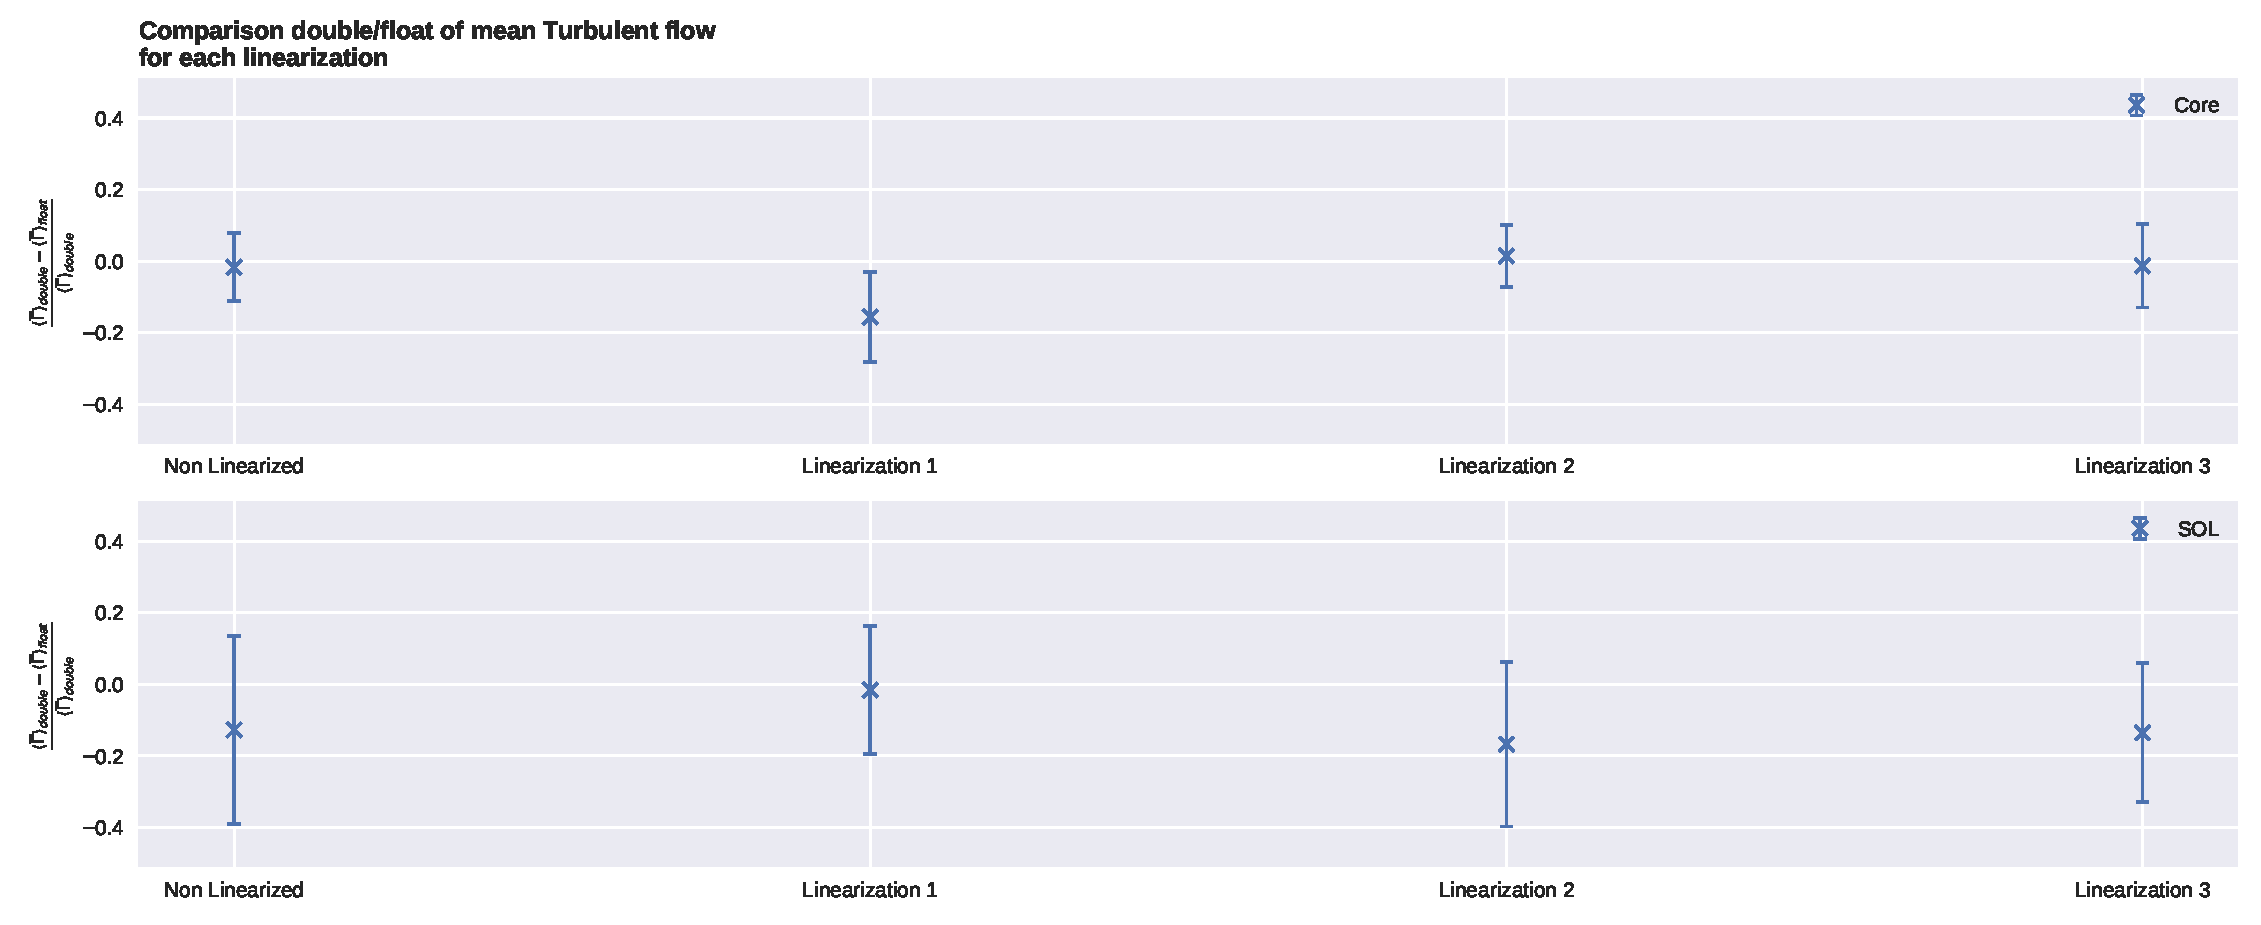
\includegraphics[width=0.32\linewidth]{pdfs/double_vs_float_80000.pdf}
    \caption{Turbulent flow float deviations from double values. The first graphic considers all iterations, the second starting from 50,000 and the last starting from 80,000. Total iterations where 100,000.}
    \label{fig:double_vs_float_all}
\end{figure}

The data shows that both precisions overall achieve almost the same value. At first a deviation of $>10\%$ may seem large but considering the fluctuations over the iterations (represented by the error bars) the results for both precisions are of the same order. For this special specific setup the \textit{float} precision does not deviate significantly from \textit{double} precision (omitting fluctuations and exact time points) hinting that the general characteristics of the model are conserved. This encourages the use of float precision if a speedup is observed. During these calculations the simulation ran about 20\% faster, but the parts involving fast fourier transformations where run in double precision since the API of the FFTW3 library does not support templating but rather as another API for float calculations. But the code could be extended to use the float version of the FFTW3 library further increasing the speedup when using float calculations. 
% Interestingly there are tendencies visible for the deviations for the different linearizations that may be connected to different gradient sizes. Higher gradients typically result into higher relative condition numbers for the derivatives (subtractions are involved) and thus more information is lost that may be compensated better by double calculations. This hints that for linearizations one and two higher gradients are present in the Core region since there the deviation between \textit{float} and \textit{double} is greater.

\end{document}
